% Allow relative paths in included subfiles that are compiled separately
% See https://tex.stackexchange.com/questions/153312/
\providecommand{\main}{..}
\documentclass[\main/thesis.tex]{subfiles}
\onlyinsubfile{\zexternaldocument*{\main/tex/introduction}}

\begin{document}

\chapter{Pipelines for Novel Drum Generation}

\label{gens}
\label{surveys}
\section{The Pipeline}
 In the previous chapter, we discussed our implementation of a \emph{virtual synthesizer}, which generates 1 second long sounds (or sonic noise) based on its parameters. We also discussed our expectations of an ideal \emph{virtual ear} along with multiple implementation attempts and measurements for accuracy. Putting these components together, we conceptualized a generative pipeline for creation of novel drum sounds, shown in figure~\ref{fig:pipeline_outline}.
 
 We expect the virtual synthesizer to make sounds, which we call \enquote{synthetic noise}. We also expect the ideal virtual synthesizer to create identical sounds, given the same program. We verified These claims in Section~\ref{chap3:synth_deterministic}. Much harder to verify are our expectations of the virtual ear. If a small subset of synthetic noise can stand in for percussive sounds, then the ideal synthetic ear will be able to the desired sounds from noise with high recall and precision. Low recall will cause a slow-down of the pipeline and loss of novel sounds. Low precision will make manual cleanup of generated samples a requirement. Critically, manual over-sight is necessary to assess the performance of the ear. 

To assess the performance of each pipeline, we randomly create drum programs and generate and the corresponding signal. This signal is then fed through the ear model to determine if the signal is percussive. If so, a category is assigned to the sound. This sound and the corresponding synthesizer program are saved to hard-disk. Here we assess the success rate of two different pipelines by manual inspection and categorization of a randomly selected subset of its results. We cross reference the manual categorizations with the categories assigned by the virtual ear: Do we agree that the sounds are percussive? Do we agree with the drum group assigned to the percussive sounds?
 
 \section{Survey of Two-Phased Ear Performance}
   
\begin{table}[htbp]
 \resizebox{\linewidth}{!}{\begin{tabular}{||c c c c c c c||} 
 \hline
 Drop Rule & Size & HvH & H+FC & H+CNN & H+E/F & 3 models \\ [0.5ex] 
 \hline
 No Drops & 257 &0.37 & 0.35 & 0.36 & 0.36 & 0.28\\ 
 \hline
 Assigned \enquote{Bad} By Both & 236 & 0.31 & 0.37 & 0.37 & 0.38 & 0.30 \\
 \hline
 Assigned \enquote{Bad} By Either & 180 & 0.47 & 0.50 & 0.48 & 0.48 &  0.34 \\
 \hline
 Assigned \enquote{Bad} or \enquote{Other} By Either & 154 & 0.47 & 0.59 & 0.54 & 0.50 &  0.35 \\
 \hline
\end{tabular}}
\caption{\label{kappa_table_TPE}Table of Fleiss' kappa coefficient to measure the degree of agreement between persons (HvH), persons with FC model (H+FC), persons with CNNLSTM model, persons with all models (H+E/F), and between the 3 models. \enquote{Drop Rule} column indicates if any samples were dropped. We show the measurements after dropping samples if they are deemed bad by either or both responders. We also show measurements after dropping the \enquote{other} category along with samples deemed bad by either responder. }
\end{table}
To measure the quality of the samples produced by our pipeline combined with the TP ear models, we run the model until an adequate number of samples in each category are saved to disk. Next, we randomly generated around 50 samples in the following categories: \enquote{snare}, \enquote{kick}, \enquote{hat}, \enquote{clap} and \enquote{other} (combination of rims, 
shakers and unusual percussive sounds). This gave us a total of 257 samples. These samples were determined to be percussive and then categorized by 3 different models (FC, CNNLSTM, E+F). We ensured a balanced division between samples of stack size 1, 2 and 4 (each stack is responsible for a third of the samples under each category). Both reviewers then categorized these samples without knowledge of other categorizations (person or computation models). It's important to note:
\begin{itemize}
    \item Each responder had an additional category of bad for samples that they deemed not percussive. The \enquote{bad} category indicates that the sample should have been skipped in Phase 1. 
    \item With 6 categorization groups, responders had the same categorization in 47\% of cases.
    \item Of 257 samples, the responders agreed with FC, CNNLSTM, and E+F respectively in 78, 76, and 46 of cases. The loss of spectrum data appears to lower performance.
\end{itemize}

\begin{figure}[h!]
    \begin{center}
    \textbf{Label Assignment Frequency}
    \makebox[\textwidth]{
    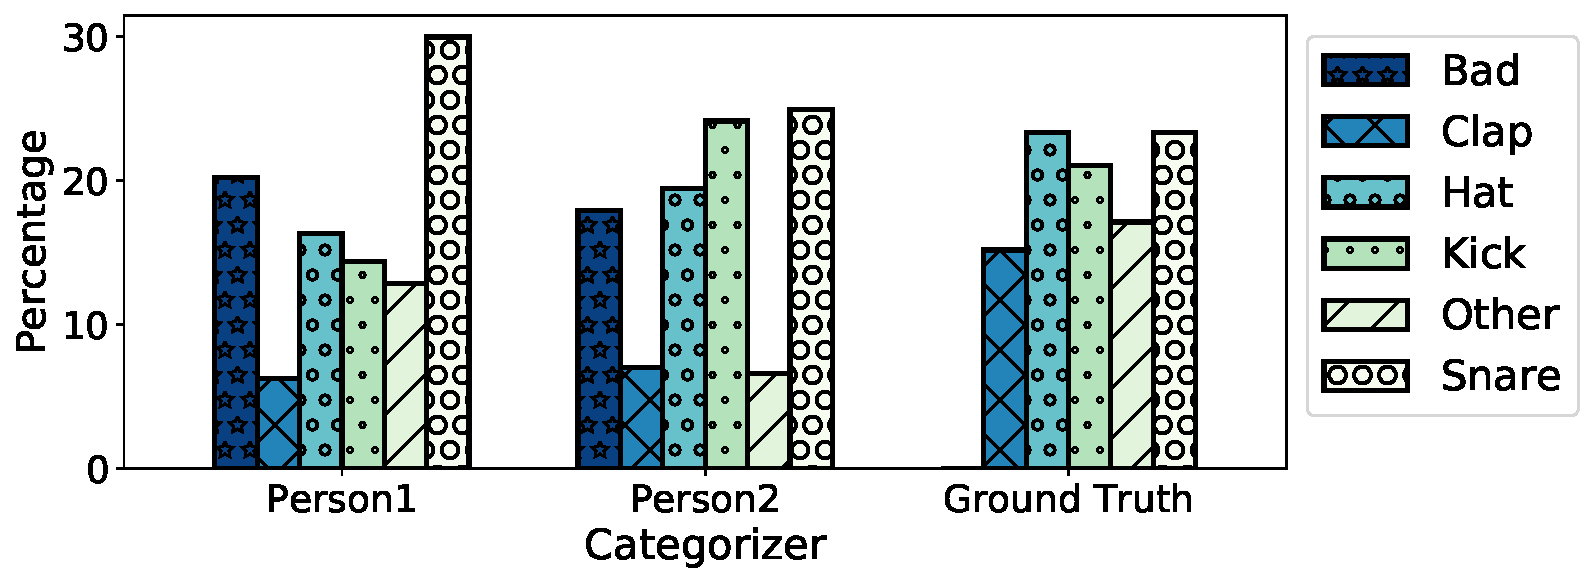
\includegraphics[width=1.1\linewidth]{images/chapter_4/cat_2p.pdf}}
    \end{center}
    \caption{Frequency of assigned labels by persons vs the true number of labels}
\label{fig:freq-survey-2p}
\end{figure}
We assess the reliability of agreement between persons and categorization models via the Fleiss' kappa coefficient \cite{fleiss1971measuring}. The value of 0 or less for this coefficient indicates no agreement beyond random chance, and the value of 1 indicating perfect agreement. Our kappa measurements showcased in~\ref{kappa_table_TPE} lie within the 0.35-0.45 range, indicating mild to moderate agreement between persons and machines. We again measure this coefficient after dropping samples that were categorized as \enquote{bad} by the authors, as samples that persons deem to be \enquote{bad} indicate a failure in Phase 1 and should not have been categorized by the models at all. Dropping of samples that both authors deemed \enquote{bad} causes an 8\% reduction of our data (21 samples) and a small increase in kappa score. Dropping samples deemed bad by either reviewer resulted in a 30\% reduction of samples and relatively large increase in kappa scores. 

\subsection{Takeaways Of The Two Phased Pipeline Survey}
\label{survey1_takeaway}
\begin{itemize}
    \item The survey brings into question the reliability of our phase 1 models, as 30\% of the generated samples were deemed not percussive by at least 1 reviewer and 8\% by both reviewers
    \item The task of categorizing synthetic drums is difficult. Survey shows that the scale of agreement within persons as well as between persons and various model combinations is moderate at best, even after removal of \enquote{bad} samples.  While the same models can easily achieve 98+ percent accuracy when tested on recorded drum samples. This may be a manifestation of the \enquote{open set recognition} problem. 
    \item While there is much room for improvement, our pipeline can generate and categorize drums and percussive sounds with a promising degree of success. 
\end{itemize}

 \section{Survey of Mixed-Models Ear Performance}
 Keeping the other components of the pipeline the same, we replace the two-phased ear in the previous pipeline with the MME. Our survey differs from the previous survey in that the pipeline only creates the four drum categories. The \enquote{other} category is only assigned by survey responders. This means that two out of six possible categories are only available to responders, therefore there is an inherent bias towards worse agreeably scores compared to last survey. Our main concern here is changes in the amount of \enquote{bad} samples. We show measurements before and after dropping all \enquote{bad} and \enquote{other} samples for a fairer comparison with the TPE pipeline.

 \begin{table}[t]
 \resizebox{\linewidth}{!}{\begin{tabular}{||c c c c||} 
 \hline
 Drop Rule & Size & HvH & H+MME \\
 \hline
 No Drop & 300 & 0.336 & 0.250\\ 
 \hline
 Assigned Bad By Both & 249 & 0.200 & 0.260 \\
 \hline
 Assigned Bad By Either & 151 & 0.460 &  0.473 \\
 \hline
Assigned \enquote{Bad} or \enquote{Other} By Either  & 120 & 0.620   &  0.587 \\
 \hline
\end{tabular}}
\caption{\label{kappa_table_MME}Table of Fleiss' kappa coefficient to measure the degree of agreement between persons (HvH) and persons and MME. We measure the agreeability scores after dropping bad samples if both or either persons assigned the sample as such. We also measure agree-ability when all samples deemed \enquote{bad} or \enquote{other} by either person are removed.}
\end{table}

\begin{figure}[htpb]
    \begin{center}
    \textbf{Category Assignment Frequency For MME Survey}
    \makebox[\textwidth]{
    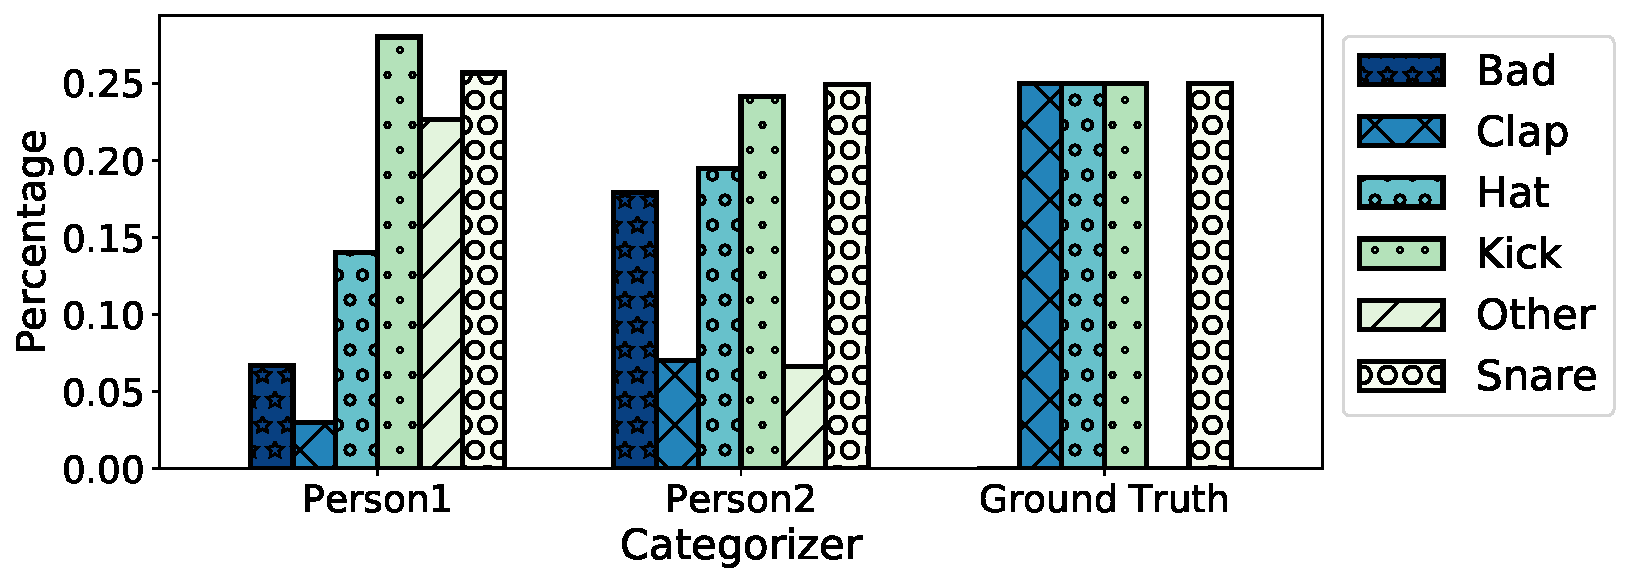
\includegraphics[width=1.1\linewidth]{images/chapter_4/cat_mme.pdf}}
    \end{center}
    \caption{Frequency of assigned labels by persons vs the true number of labels}
\label{fig:freq-survey-2p}
\end{figure} 
\subsection{Takeaways Of The MME Pipeline Survey}
\label{survey2_takeaway}
The results from the two surveys are not easily comparable. However, no major improvements in agree-ability or a decrease in the number of bad samples can be seen, in fact, the opposite is more likely to be true. However, we are yielding comparable results to the TPE pipeline despite having a fraction of the features to learn from (latent layer + 10 envelope features). Suggesting that latent representations of autoencoder networks can be used as general, low-dimensional proxies for representation of complex inputs. 

Agree-ability scores for MME pipeline are often lower, but we reiterate that this can be caused by having two out of six (rather than one out of six in the TPE pipeline) categories which are exclusive to survey responders. Supporting this hypothesis is the notable improvement in agree-ability observed after dropping all \enquote{bad} and \enquote{other} samples. Here, both persons agree with each other and with the MME at a stronger rate than in the TPE pipeline, despite having similar number of samples (120 for MME and 154 for TPE) and equal number of categories to choose from. This values are observed in the last rows of tables~\ref{kappa_table_TPE} and ~\ref{kappa_table_MME}. The higher DVD categorization accuracy achieved by the mixed-model ear compared to the best two-phaaed ear is consistent with this observation: Given that the sound being categorized is a drum, the MME will yield better results that the TPE. However, the MME pipeline does not yield better results in the DVN task. 


% \section{Genetic Search}
% %  introduce genetic search and how it works for our project
% % 3 graphs for 3 stack sizes trying to find a certain type of drum
%  \section{Speed}
%  With our current models, a single iteration of this pipeline will take approximately 50 milliseconds for Synthesizers with stack sizes of 8 or less. This means around 20 iterations can be done per second using a single process. This pipeline scales up efficiently with multiprocessing. We have not measured the iteration latency for this pipeline when a GPU is leveraged. For reference, our CPU measurements are collected on a 2012 Macbook Air running Ubuntu 18.04.
\end{document}